\documentclass{beamer}  
\usetheme{Warsaw}
\usepackage{amsmath}
\title{Introduction to AI and ML}
\subtitle{Google PageRank}
\author{Manideep, EE17BTECH11046 \\ Yashas, ES17BTECH11025}
\begin{document}

\begin{frame}

\titlepage
 
\end{frame} 
 
\begin{frame}{Google PageRank Algorithm}
From the previous presentation:\\
\[
PR(p_{i};t+1)=\dfrac{1-d}{N} + d
    \sum_{p_{j} \epsilon M(p_{i})}\dfrac{PR(p_{j};t)}{L(p_{j})}
\]
where $p_{1}, p_{2} , . . . , p_{N}$ are the pages under consideration,\\
$M(p_{i})$ is the set of pages that link to $p_{i}$,\\
$d$ is damping factor,(generally,d=0.85),\\
$L(p_{j})$ is the number of outbound links on page $p_{j}$,\\
and $N$ is the total number of pages.
\end{frame}

\begin{frame}{Matrix Form}
\footnotesize
\setlength{\arraycolsep}{9pt}
\medmuskip = 1mu
The PageRank matrix R,is represented as:
\[
\textbf{R}=
\begin{bmatrix}
PR(p_{1})\\
PR(p_{1})\\
\vdots	\\
PR(p_{N})\\
\end{bmatrix}
\]
\hspace{-30em}
\[
\textbf{R}(t+1)=
\begin{bmatrix}
(1-d)/N \\
(1-d)/N \\
\vdots	\\
(1-d)/N \\
\end{bmatrix}
+ d\begin{bmatrix}
l(p_{1},p_{1}) &l(p_{1},p_{2})&\cdots &	l(p_{1},p_{N})\\
l(p_{2},p_{1})& \ddots & &l(p_{2},p{N})\\
\vdots& &l(p_{i},p_{j}) & \vdots\\
l(p_{N},p_{1}) & l(p_{N},p_{2})&\cdots &l(p_{N},p_{N})\\
\end{bmatrix}
\textbf{R}(t)
\]
\vspace{1em}
where the adjacency function\\
$l(p_{i},p_{j})=$ is
$
\begin{cases}
\dfrac{1}{L(p_{j})} & ,$if j links to i$\\
0 & ,$otherwise$
\end{cases}
$\\
\end{frame}

\begin{frame}
\[
\sum_{i=1}^{N} l(p_{i},p_{j})=1
\]
i.e. the elements of each column sum up to 1 \\
\vspace{2.5em}
\hspace{2em}As a result of Markov theory, it can be shown that the PageRank of a page is the probability of arriving at that page after a large number of clicks.\\
\vspace{2.5em}
Now t $\rightarrow \infty$ \textbf{R(t)}=\textbf{R} is the required solution 
\end{frame}

\begin{frame}{Web Graph}
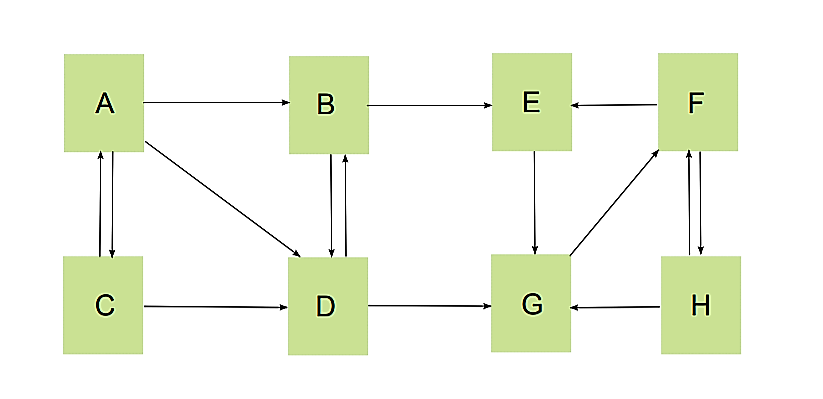
\includegraphics[scale=0.5]{Pages.png}
\end{frame}

\begin{frame}{Methods of calculating PageRank}
\begin{itemize}
\item{Algebraic Method}
\item{Power Method}
\end{itemize}
\end{frame}

\begin{frame}{Algebraic Method}
We have:
\[
\textbf{R}(t+1)=
\dfrac{1-d}{N}\textbf{1}
+ d\mathcal{M}
\textbf{R}(t)
\]
where:\\

$\mathcal{M}_{ij}=$ is
$
\begin{cases}
\dfrac{1}{L(p_{j})} & ,$if j links to i$\\
0 & ,$otherwise$
\end{cases}
$\\
\vspace{1.5em}
\textbf{1} is the column vector of length $N$ containing only ones.\\


\end{frame}
\begin{frame}{Algebraic Method}
As t $\rightarrow \infty$ :
\[
\textbf{R}=d\mathcal{M}\textbf{R} + \dfrac{1-d}{N}\textbf{1}
\]

\[
\textbf{R}=(\textbf{I} - d\mathcal{M})^{-1} \dfrac{(1-d)}{N}\textbf{1}
\]
We have the constraint that sum of elements of \textbf{R} is 1.\\
So by normalizing it,
\[
\textbf{R}_{a}=\dfrac{\textbf{R}}{||\textbf{R}||}
\]
\end{frame}

\begin{frame}
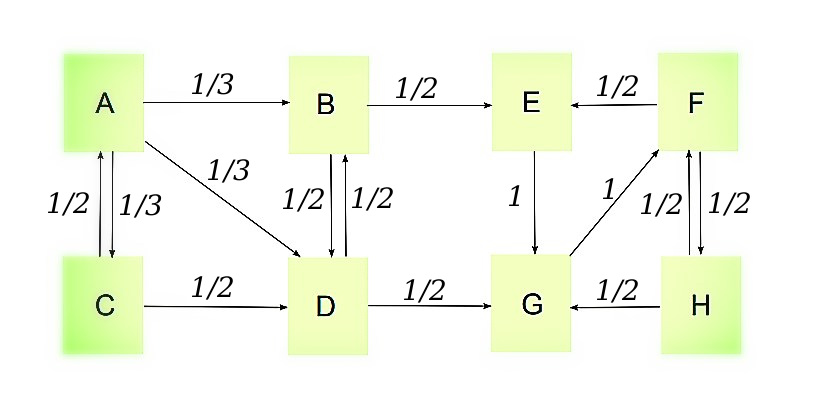
\includegraphics[scale=0.4]{Pagerank.jpg}
\end{frame}
\begin{frame}
\footnotesize
\setlength{\arraycolsep}{6.8pt}
\medmuskip = 1mu
Now we have,$\mathcal{M}=$
\[
\begin{bmatrix}
0 & 0 & 1/2 & 0 & 0 & 0 & 0 & 0\\ 
1/3 & 0 & 0 & 1/2 & 0 & 0 & 0 & 0\\ 
1/3 & 0 & 0 & 0 & 0 & 0 & 0 & 0\\ 
1/3 & 1/2 & 1/2 & 0 & 0 & 0 & 0 & 0\\ 
0 & 1/2 & 0 & 0 & 0 & 1/2 & 0 & 0\\ 
0 & 0 & 0 & 0 & 0 & 0 & 1 & 1/2\\ 
0 & 0 & 0 & 1/2 & 1 & 0 & 0 & 1/2\\ 
0 & 0 & 0 & 0 & 0 & 1/2 & 0 & 0\\ 
\end{bmatrix}
\]
$N= 8$\\
$d=0.85$\\
\vspace{1em}
Substituting the above values in the equation we get:
\[
\textbf{R}_{a}=
\begin{bmatrix}
0.0304 & 0.0536& 0.0274 & 0.0618& 0.1621& 0.2836& 0.2419&0.1393
\end{bmatrix}^T
\]
\end{frame}


\begin{frame}{Power Method}
\[
\textbf{R}=(d\mathcal{M}+\dfrac{1-d}{N}\textbf{E})\textbf{R}
\]
where \textbf{E} is the matrix whose elements are all 1.(Here,\textbf{ER}=\textbf{1})\\
Here we are making a constraint that sum of all PageRanks is 1\\
\vspace{1em}
Writing $(d\mathcal{M}+\dfrac{1-d}{N}\textbf{E})$ as the operator $\widehat{\mathcal{M}}$:
\[
\textbf{R}=\widehat{\mathcal{M}}\textbf{R}
\]
\end{frame}

\begin{frame}
The power method involves applying the operator $\widehat{\mathcal{M}}$ in succession on the required vector.If the vector under consideration is $x(t)$ which starts from $x(0)$ (normalized vector):
\[
x(t+1)=\widehat{\mathcal{M}}x(t)
\]
This is done until:
\[
|x(t+1)-x(t)| < \epsilon
\]

After some finite number of iterations based on the value of $\epsilon$ ,we get the matrix \textbf{R}.\\
\vspace{1em}
Taking $\epsilon$ as $10^{-8}$ 
\[
\textbf{R}=
\begin{bmatrix}
.0304 & .0536& .0274 & .0618& .1623& .2834& .2416&.1393
\end{bmatrix}^T
\]
\end{frame}

%\begin{frame}
%The above two computations using $\mathcal{M}$ only give the same PageRank %if their results are normalized:
%\[
%\textbf{R}_{power}=\dfrac{\textbf{R}_{algebraic}}{|\textbf{R}_{algebraic}|}
%\]
%\end{frame}

\end{document}